\documentclass[11pt,a4paper]{article}

% ------------------------------------------------------------------
\usepackage[margin=2.3cm]{geometry}
\usepackage{fontspec}
\setmainfont{TeX Gyre Termes}
\usepackage{titlesec}
\usepackage{xcolor}
\definecolor{hxblue}{RGB}{27,54,93}
\definecolor{hxgrey}{RGB}{90,90,90}
\definecolor{hxlight}{RGB}{235,240,247}
\definecolor{codebg}{RGB}{245,246,248}
\usepackage{booktabs}
\usepackage{longtable}
\usepackage{array}
\usepackage{enumitem}
\usepackage{fancyhdr}
\usepackage{hyperref}
\usepackage{caption}
\usepackage{parskip}
\usepackage{tikz}
\usetikzlibrary{shapes.geometric,arrows.meta,positioning,calc,fit}

\hypersetup{
  colorlinks=true,
  linkcolor=hxblue,
  citecolor=hxblue,
  urlcolor=hxblue,
  pdftitle={HypatiaX Hybrid Variants -- Naming, Experiment Map \& Algorithm Diagrams},
  pdfauthor={Claude (Anthropic) -- Automated Code Analysis}
}

\titleformat{\section}{\Large\bfseries\color{hxblue}}{\thesection}{0.6em}{}
\titleformat{\subsection}{\large\bfseries\color{hxblue}}{\thesubsection}{0.6em}{}
\titleformat{\subsubsection}{\normalsize\bfseries\color{hxgrey}}{\thesubsubsection}{0.6em}{}

\pagestyle{fancy}
\fancyhf{}
\renewcommand{\headrulewidth}{0.4pt}
\lhead{\small\color{hxgrey} HypatiaX Hybrid Variants -- Naming, Experiment Map \& Algorithms}
\rhead{\small\color{hxgrey}\thepage}

\newcommand{\repolink}{\url{https://github.com/sednabcn/LLM-HypatiaX-REPRO}}
\newcommand{\code}[1]{\texttt{\small #1}}

% ---- tikz styles for flowcharts ----
\tikzset{
  proc/.style={draw, rounded corners, fill=hxblue!8, align=center, minimum width=4.6cm, minimum height=0.9cm, font=\small},
  stage/.style={draw, rounded corners, fill=hxblue!16, align=center, minimum width=4.6cm, minimum height=0.9cm, font=\small\bfseries},
  dec/.style={draw, diamond, aspect=3.6, fill=hxblue!28, align=center, inner sep=2pt, font=\scriptsize},
  outp/.style={draw, rounded corners, fill=hxblue!45, align=center, minimum width=4.2cm, minimum height=0.9cm, font=\small\bfseries},
  arr/.style={-Latex, thick},
  lbl/.style={font=\scriptsize\color{hxgrey}}
}

\begin{document}

% ==================================================================
\begin{titlepage}
\centering
\vspace*{1.5cm}
{\Huge\bfseries\color{hxblue} HypatiaX Hybrid Variants}\\[0.4cm]
{\Large Naming, Experiment Cross-Reference \& Algorithm Diagrams}\\[1.2cm]
{\large Source repository: \repolink\ (\code{master})}\\[0.3cm]
{\large Built on the prior static-analysis report (\code{core/}, \code{experiments/}, \code{tools/}, \code{protocols/})}\\[2cm]

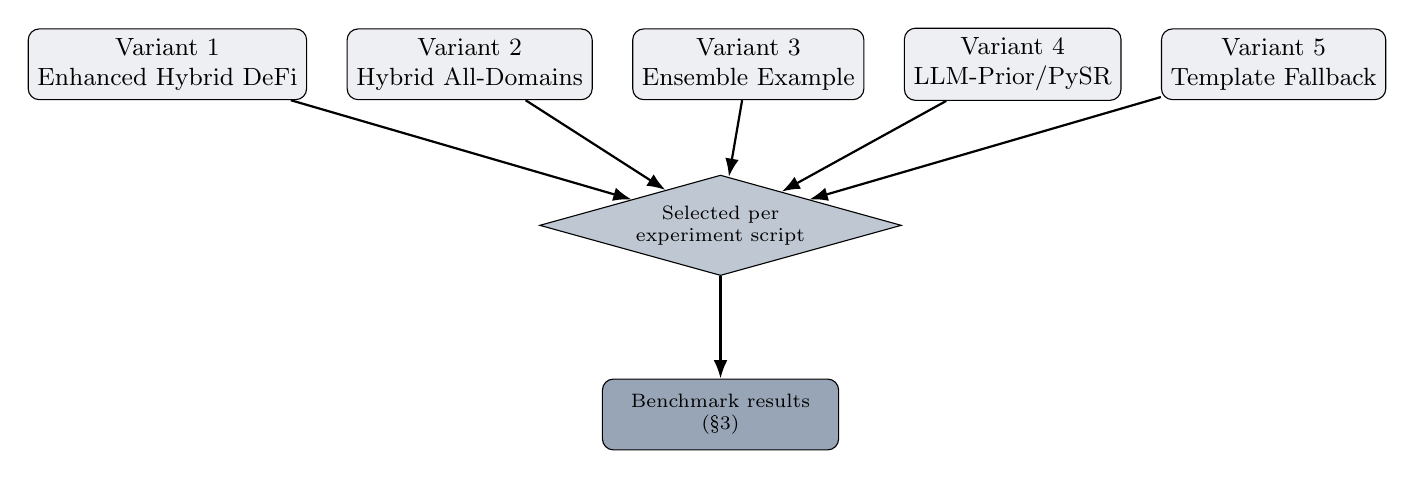
\begin{tikzpicture}[node distance=0.9cm and 0.5cm, every node/.style={font=\tiny}]
  \node[proc, minimum width=2.1cm, minimum height=0.8cm] (v1) {Variant 1\\Enhanced Hybrid DeFi};
  \node[proc, minimum width=2.1cm, minimum height=0.8cm, right=of v1] (v2) {Variant 2\\Hybrid All-Domains};
  \node[proc, minimum width=2.1cm, minimum height=0.8cm, right=of v2] (v3) {Variant 3\\Ensemble Example};
  \node[proc, minimum width=2.1cm, minimum height=0.8cm, right=of v3] (v4) {Variant 4\\LLM-Prior/PySR};
  \node[proc, minimum width=2.1cm, minimum height=0.8cm, right=of v4] (v5) {Variant 5\\Template Fallback};
  \node[dec, below=1.4cm of $(v1)!0.5!(v5)$, minimum width=3.0cm, font=\scriptsize] (dec) {Selected per\\experiment script};
  \node[outp, below=1.3cm of dec, minimum width=3.0cm, font=\scriptsize] (out) {Benchmark results\\(\S3)};
  \draw[arr] (v1) -- (dec); \draw[arr] (v2) -- (dec); \draw[arr] (v3) -- (dec);
  \draw[arr] (v4) -- (dec); \draw[arr] (v5) -- (dec);
  \draw[arr] (dec) -- (out);
\end{tikzpicture}

\vfill
{\large Prepared by: Claude (Anthropic), automated repository analysis}\\
{\large \today}
\end{titlepage}

\tableofcontents
\newpage

% ==================================================================
\section{1) Variant list and naming}
% ==================================================================
Five hybridisation \emph{variants} exist across \code{hypatiax/core/} and
\code{hypatiax/tools/}. Each implements a different way of combining an
LLM-generated symbolic prior with a numeric predictor (neural network,
genetic-programming symbolic regression, or a template library). Table~1
names each one and gives its defining class, its combination strategy, and
where it lives in the repository.

\begin{table}[h!]
\centering
\renewcommand{\arraystretch}{1.3}
\begin{tabular}{@{}p{0.6cm}p{4.0cm}p{4.6cm}p{4.6cm}@{}}
\toprule
\textbf{\#} & \textbf{Name} & \textbf{Defining class / function} & \textbf{Combination strategy} \\
\midrule
1 & Enhanced Hybrid DeFi & \code{EnhancedHybridSystemDeFi} & Fixed $R^2\!\geq\!0.85$ + margin$>0.05$ threshold gate, after a \code{scipy.optimize.curve\_fit} constant refit of the LLM formula \\
2 & Hybrid All-Domains & \code{HybridSystemAllDomains} & Tie-favours-symbolic gate ($r2_{llm}\!\geq\!r2_{nn}$), with a \code{force\_llm} override that skips the NN for known power-law domains \\
3 & Ensemble Example & \code{ensemble\_llm\_nn()} & Precision-weighted blend: weight $\propto R^2/\sigma_{resid}$ (inverse-residual-std), no hard gate \\
4 & LLM-Prior / PySR Family & \code{SymbolicEngineWithLLM} (4 modes: \code{none}/\code{seed}/\code{hybrid}/\code{fallback}), driven by \code{HybridDiscoverySystem} & LLM and genetic-programming (PySR) take turns proposing/refining one candidate expression \\
5 & Template Physics Fallback & \code{PhysicsAwareRegressor} (template-library) / \code{SmartStructureDetector} (template-free) & Fits a library of domain-specific forms (Michaelis-Menten, Bernoulli, \ldots) or infers additive/multiplicative structure statistically, used when Variant~4 underperforms \\
\bottomrule
\end{tabular}
\caption{The five HypatiaX hybrid variants.}
\end{table}

\subsection{Where each variant lives}
\begin{itemize}[leftmargin=1.3cm]
  \item[\code{[C1]}] \code{hypatiax/core/generation/hybrid\_defi\_system/hybrid\_system\_nn\_defi\_domain.py} -- Variant 1
  \item[\code{[C2]}] \code{hypatiax/core/generation/hybrid\_all\_domains\_llm\_nn/hybrid\_system\_llm\_nn\_all\_domains.py} -- Variant 2
  \item[\code{[C3]}] \code{hypatiax/core/generation/hybrid\_defi\_llm\_nn/hybrid\_ensemble\_system\_defi\_domain.py} -- Variant 3
  \item[\code{[T1]/[T2]}] \code{hypatiax/tools/symbolic/hybrid\_system\_v50\_2.py} (orchestrator) / \code{symbolic\_engine.py} (mode logic) -- Variant 4
  \item[\code{[T3]/[T4]}] \code{hypatiax/tools/symbolic/physics\_aware\_regressor.py} / \code{smart\_structure\_detector.py} -- Variant 5
\end{itemize}

\newpage
% ==================================================================
\section{2) Variant $\to$ experiment cross-reference}
% ==================================================================
Table~2 links each variant to the experiment scripts in
\code{hypatiax/experiments/benchmarks/} and \code{hypatiax/experiments/tests/}
that actually construct or import it, confirmed by direct source
inspection (class names / imports found in each file).

\begin{longtable}{@{}p{2.6cm}p{6.3cm}p{6.3cm}@{}}
\toprule
\textbf{Variant} & \textbf{Experiment file(s)} & \textbf{Evidence (import / usage found)} \\
\midrule
\endhead
1. Enhanced Hybrid DeFi &
  \code{hypatiax\_defi\_benchmark\_v4.py} (run directly by the \code{exp1}/\code{exp1b} pipeline steps, Tab 9-15), \code{run\_comparative\_suite\_benchmark\_v2.py}, \code{\_pca.py}, \code{run\_noise\_sweep\_benchmark.py}, \code{run\_sample\_complexity\_benchmark.py}, \code{test\_enhanced\_defi\_extrapolation.py} &
  \code{run\_all.sh}'s \code{exp1}/\code{exp1b} steps invoke \code{hypatiax\_defi\_benchmark\_v4.py} directly as the paper's core DeFi benchmark (which itself calls \code{EnhancedHybridSystemDeFi}); \code{run\_noise\_sweep\_benchmark.py} and \code{run\_sample\_complexity\_benchmark.py} name it explicitly as ``method 3'' \\
\midrule
2. Hybrid All-Domains &
  \code{hybrid\_system\_llm\_nn\_all\_domains.py} (run directly as \code{hybrid\_all\_domains} pipeline step), \code{run\_sample\_complexity\_benchmark.py}, \code{run\_comparative\_suite\_benchmark\_v2.py}/\code{\_pca.py} &
  \code{run\_all.sh}'s \code{hybrid\_all\_domains} step (\S10.9) \code{cd}s into \code{hybrid\_all\_domains\_llm\_nn/} and runs \code{hybrid\_system\_llm\_nn\_all\_domains.py} directly -- the clearest evidence of any variant, since this is Variant 2's own defining file executed as the experiment; \code{run\_sample\_complexity\_benchmark.py} names \code{HybridSystemLLMNN all-domains} alongside Variant 1 \\
\midrule
3. Ensemble Example &
  \code{hypatiax\_defi\_benchmark\_v3.py}, \code{\_v4.py}, \code{\_v3\_pca.py}, \code{\_v4\_pca.py}, \code{test\_enhanced\_defi\_extrapolation.py} &
  Each defines/calls a local \code{\_ensemble\_llm\_nn()} function; \code{test\_enhanced\_defi\_extrapolation.py} imports \code{ensemble\_llm\_nn} directly and calls it -- so, despite being introduced as a ``worked example'', this variant \emph{is} exercised in the DeFi v3/v4 benchmark family and its tests \\
\midrule
4. LLM-Prior / PySR Family &
  \code{hypatia.py}, \code{exp1\_ablation.py} (run by pipeline step \code{exp1\_ablation}, Tab 5, \S10.6), \code{exp1\_five\_system.py} (step \code{exp1\_five}, Tab 1, \S10.1), \code{exp3\_nguyen12\_consolidated.py} (step \code{exp3}, \S10.8), \code{run\_comparative\_suite\_benchmark\_v2.py}/\code{\_pca.py} &
  \code{hypatia.py} defines \code{get\_llm\_prior()} directly; \code{exp1\_ablation.py} and \code{exp1\_five\_system.py} import \code{HybridDiscoverySystem} (which wraps \code{SymbolicEngineWithLLM}) and are run by \code{run\_all.sh} with \code{ANTHROPIC\_API\_KEY} required; \code{exp3\_nguyen12\_consolidated.py} imports \code{get\_llm\_prior} from \code{hypatia}; the comparative-suite scripts import \code{SymbolicEngineWithLLM} and \code{HybridDiscoverySystem} by name \\
\midrule
5. Template Physics Fallback &
  \code{exp1\_ablation.py}, \code{run\_comparative\_suite\_benchmark\_v2.py}/\code{\_pca.py} (indirectly, via \code{HybridDiscoverySystem}) &
  Not imported directly by any experiment script; reached only as an internal fallback tier inside \code{HybridDiscoverySystem} \code{[T1]} when its PySR/LLM search underperforms -- so it is exercised only transitively, wherever Variant~4 is exercised \\
\bottomrule
\caption{Variant $\to$ experiment mapping, from direct source inspection.}
\end{longtable}

\noindent\textit{Note:} \code{run\_hybrid\_system\_benchmark.py}, \code{run\_instability\_suite.py} and the
\code{portfolio\_variance\_v3c2.py}/\code{\_v4c2.py} audit scripts were also read but showed no
direct class-level reference to a specific variant at the top-level scope
searched (they either re-import from the DeFi v3/v4 modules above or operate
on already-produced result files), so they are omitted from Table~2 to avoid
overstating the evidence.

\noindent\textit{Additional evidence source:} the master orchestration script
\code{run\_all.sh} (uploaded separately, not in the \code{master} tree) lists
the full pipeline as an ordered sequence of named steps (\code{exp1},
\code{exp1b}, \code{exp1\_ablation}, \code{exp1\_five}, \code{hybrid\_all\_domains},
\code{exp2\_feynman}, \code{exp3}, \code{exp3b}, \code{suppA}, \code{suppB},
\ldots), each invoking one or more of the experiment scripts above with
explicit paths and environment variables (e.g.\ \code{PYSR\_POPULATIONS},
\code{METHOD\_TIMEOUT}, \code{ANTHROPIC\_API\_KEY} implied by \code{exp1\_ablation}'s
own warning text). Two points from it materially strengthen Table~2:
\begin{itemize}[leftmargin=1.3cm]
  \item the \code{hybrid\_all\_domains} step (\S10.9 of the paper) \code{cd}s
        directly into \code{hybrid\_all\_domains\_llm\_nn/} and runs
        \code{hybrid\_system\_llm\_nn\_all\_domains.py} as a standalone script --
        i.e.\ Variant~2's own file \emph{is} the experiment, not merely
        imported by one;
  \item the \code{exp1}/\code{exp1b} steps run \code{hypatiax\_defi\_benchmark\_v4.py}
        directly as the paper's core DeFi benchmark (Tab.\ 9--15), confirming
        Variant~1 (and, via its internal \code{\_ensemble\_llm\_nn}, Variant~3)
        as production-path code rather than illustrative-only.
\end{itemize}

\newpage
% ==================================================================
\section{3) Algorithm diagrams}
% ==================================================================

\subsection{Variant 1 -- Enhanced Hybrid DeFi (\code{EnhancedHybridSystemDeFi})}
\begin{center}
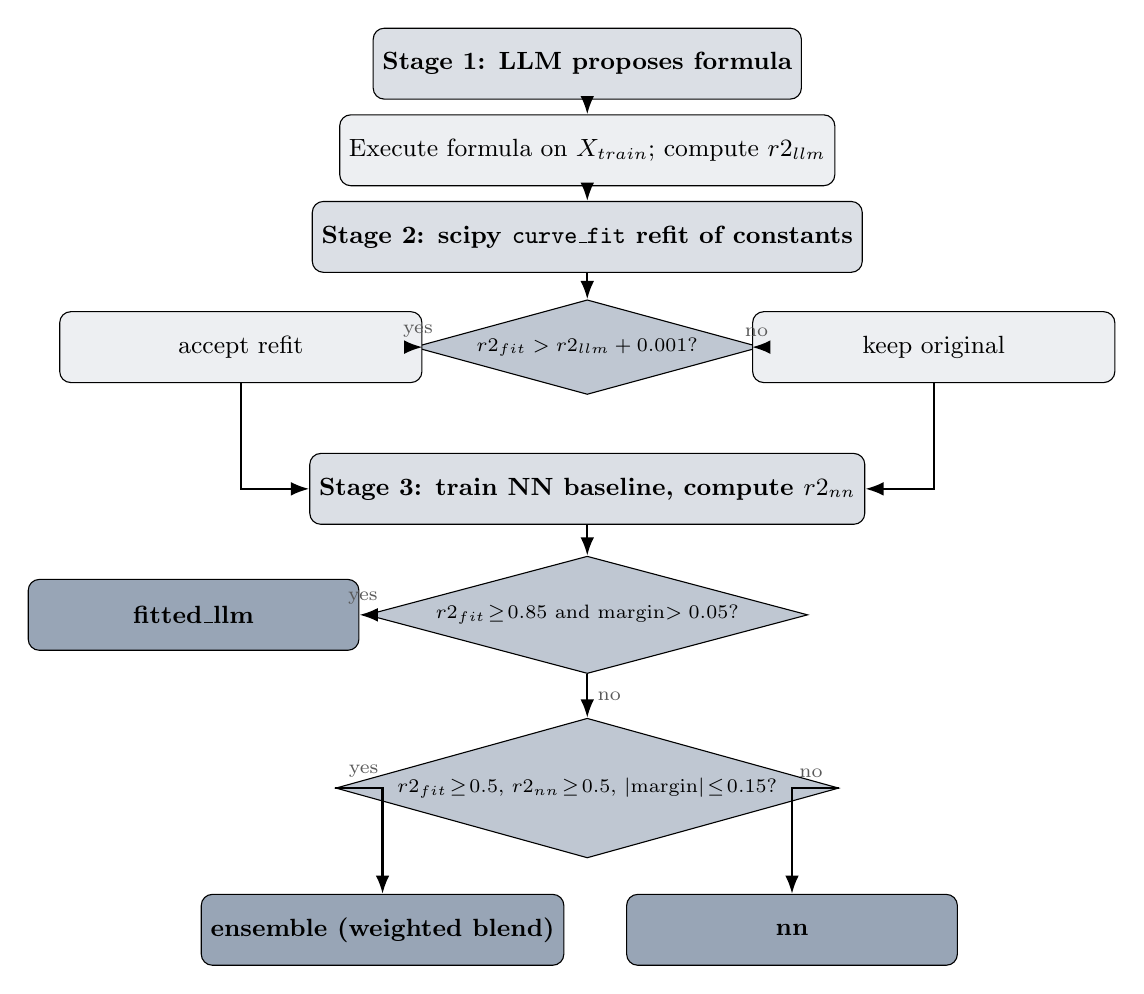
\begin{tikzpicture}[node distance=0.75cm and 1.2cm, every node/.style={font=\small}]
  \node[stage] (s1) at (0,0) {Stage 1: LLM proposes formula};
  \node[proc] (s1b) at (0,-1.1) {Execute formula on $X_{train}$; compute $r2_{llm}$};
  \node[stage] (s2) at (0,-2.2) {Stage 2: scipy \code{curve\_fit} refit of constants};
  \node[dec, minimum width=4.4cm] (d1) at (0,-3.6) {$r2_{fit} > r2_{llm}+0.001$?};
  \node[proc] (y1) at (-4.4,-3.6) {accept refit};
  \node[proc] (n1) at (4.4,-3.6) {keep original};
  \node[stage] (s3) at (0,-5.4) {Stage 3: train NN baseline, compute $r2_{nn}$};
  \node[dec, minimum width=5.6cm] (gate) at (0,-7.0) {$r2_{fit}\!\geq\!0.85$ and margin$>0.05$?};
  \node[outp] (o1) at (-5.0,-7.0) {fitted\_llm};
  \node[dec, minimum width=5.4cm] (gate2) at (0,-9.2) {$r2_{fit}\!\geq\!0.5$, $r2_{nn}\!\geq\!0.5$, $|$margin$|\!\leq\!0.15$?};
  \node[outp] (o2) at (-2.6,-11.0) {ensemble (weighted blend)};
  \node[outp] (o3) at (2.6,-11.0) {nn};
  \draw[arr] (s1) -- (s1b);
  \draw[arr] (s1b) -- (s2);
  \draw[arr] (s2) -- (d1);
  \draw[arr] (d1) -- node[lbl, above]{yes} (y1);
  \draw[arr] (d1) -- node[lbl, above]{no} (n1);
  \draw[arr] (y1) |- (s3);
  \draw[arr] (n1) |- (s3);
  \draw[arr] (s3) -- (gate);
  \draw[arr] (gate) -- node[lbl, above]{yes} (o1);
  \draw[arr] (gate) -- node[lbl, right]{no} (gate2);
  \draw[arr] (gate2) -| node[lbl, pos=0.3, above]{yes} (o2);
  \draw[arr] (gate2) -| node[lbl, pos=0.3, above]{no} (o3);
\end{tikzpicture}
\end{center}

\subsection{Variant 2 -- Hybrid All-Domains (\code{HybridSystemAllDomains})}
\begin{center}
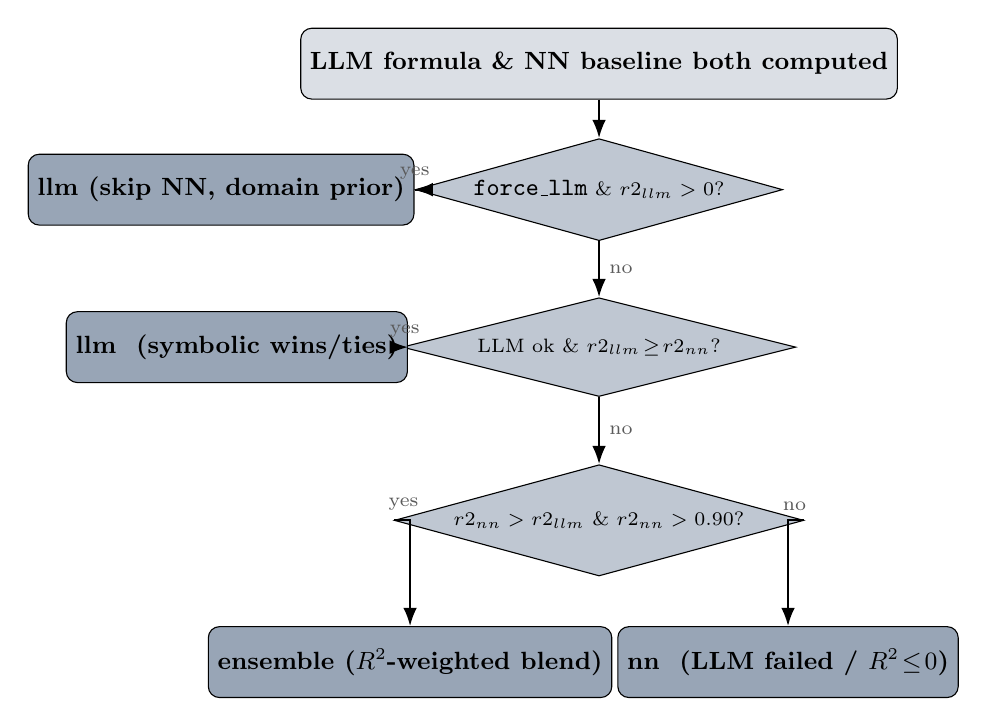
\begin{tikzpicture}[every node/.style={font=\small}]
  \node[stage] (s1) at (0,0) {LLM formula \& NN baseline both computed};
  \node[dec, minimum width=4.6cm] (fl) at (0,-1.6) {\code{force\_llm} \& $r2_{llm}>0$?};
  \node[outp] (o0) at (-4.8,-1.6) {llm (skip NN, domain prior)};
  \node[dec, minimum width=5.0cm] (d1) at (0,-3.6) {LLM ok \& $r2_{llm}\!\geq\!r2_{nn}$?};
  \node[outp] (o1) at (-4.6,-3.6) {llm\ \ (symbolic wins/ties)};
  \node[dec, minimum width=5.2cm] (d2) at (0,-5.8) {$r2_{nn}>r2_{llm}$ \& $r2_{nn}>0.90$?};
  \node[outp] (o2) at (-2.4,-7.6) {ensemble ($R^2$-weighted blend)};
  \node[outp] (o3) at (2.4,-7.6) {nn\ \ (LLM failed / $R^2\!\leq\!0$)};
  \draw[arr] (s1) -- (fl);
  \draw[arr] (fl) -- node[lbl, above]{yes} (o0);
  \draw[arr] (fl) -- node[lbl, right]{no} (d1);
  \draw[arr] (d1) -- node[lbl, above]{yes} (o1);
  \draw[arr] (d1) -- node[lbl, right]{no} (d2);
  \draw[arr] (d2) -| node[lbl, pos=0.3, above]{yes} (o2);
  \draw[arr] (d2) -| node[lbl, pos=0.3, above]{no} (o3);
\end{tikzpicture}
\end{center}

\subsection{Variant 3 -- Ensemble Example (\code{ensemble\_llm\_nn})}
\begin{center}
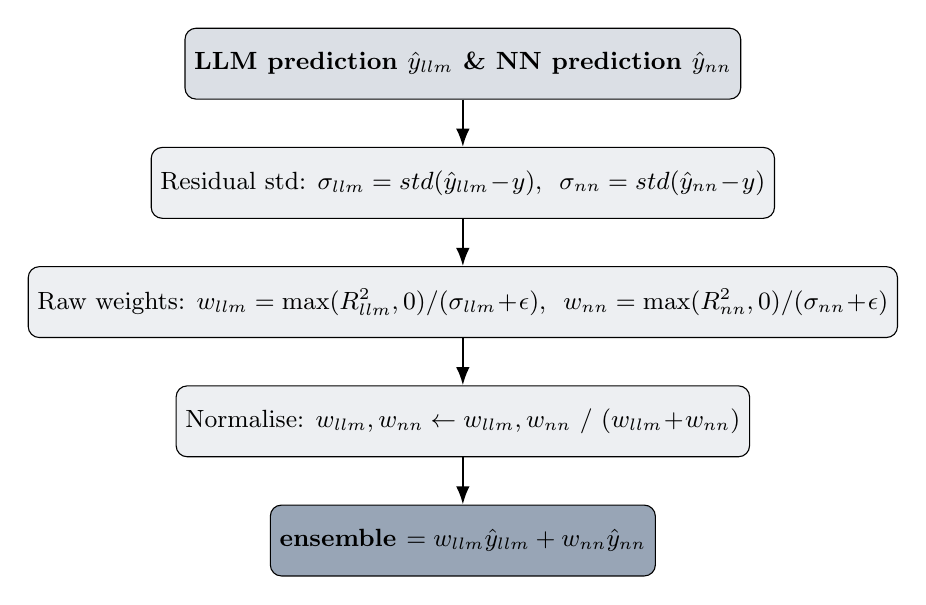
\begin{tikzpicture}[node distance=0.6cm and 1.2cm]
  \node[stage] (s1) {LLM prediction $\hat{y}_{llm}$ \& NN prediction $\hat{y}_{nn}$};
  \node[proc, below=of s1] (s2) {Residual std: $\sigma_{llm}=\text{std}(\hat{y}_{llm}\!-\!y)$,\ \ $\sigma_{nn}=\text{std}(\hat{y}_{nn}\!-\!y)$};
  \node[proc, below=of s2] (s3) {Raw weights: $w_{llm}=\max(R^2_{llm},0)/(\sigma_{llm}\!+\!\epsilon)$,\ \ $w_{nn}=\max(R^2_{nn},0)/(\sigma_{nn}\!+\!\epsilon)$};
  \node[proc, below=of s3] (s4) {Normalise: $w_{llm},w_{nn}\gets w_{llm},w_{nn}\ /\ (w_{llm}\!+\!w_{nn})$};
  \node[outp, below=of s4] (o1) {ensemble $= w_{llm}\hat{y}_{llm} + w_{nn}\hat{y}_{nn}$};
  \draw[arr] (s1) -- (s2);
  \draw[arr] (s2) -- (s3);
  \draw[arr] (s3) -- (s4);
  \draw[arr] (s4) -- (o1);
\end{tikzpicture}
\end{center}
No hard decision gate: this variant always returns a precision-weighted blend of both models' predictions.

\newpage
\subsection{Variant 4 -- LLM-Prior / PySR Family (\code{SymbolicEngineWithLLM}, mode-dispatched)}
\begin{center}
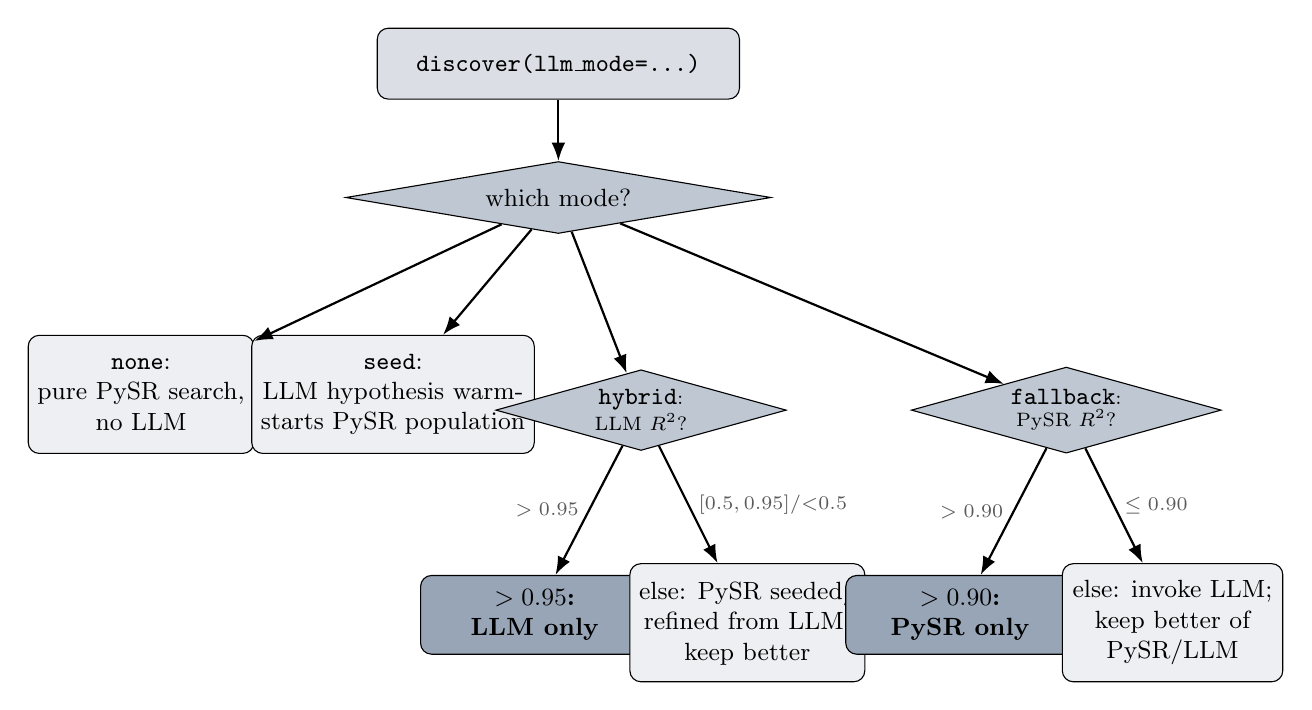
\begin{tikzpicture}[every node/.style={font=\scriptsize}]
  \node[stage, font=\small] (s1) at (1.9,0) {\code{discover(llm\_mode=...)}};
  \node[dec, minimum width=5.4cm, font=\small] (m) at (1.9,-1.7) {which mode?};
  \node[proc, minimum width=2.5cm, minimum height=1.5cm] (none) at (-3.4,-4.2) {\code{none}:\\pure PySR search,\\no LLM};
  \node[proc, minimum width=2.5cm, minimum height=1.5cm] (seed) at (-0.2,-4.2) {\code{seed}:\\LLM hypothesis warm-\\starts PySR population};
  \node[dec, minimum width=2.8cm] (hyb) at (2.95,-4.4) {\code{hybrid}:\\LLM $R^2$?};
  \node[dec, minimum width=2.8cm] (fb) at (8.35,-4.4) {\code{fallback}:\\PySR $R^2$?};
  \node[outp, minimum width=2.9cm, minimum height=1.0cm] (hyb1) at (1.6,-7.0) {$>0.95$:\\LLM only};
  \node[proc, minimum width=2.8cm, minimum height=1.5cm] (hyb2) at (4.3,-7.1) {else: PySR seeded/\\refined from LLM;\\keep better};
  \node[outp, minimum width=2.9cm, minimum height=1.0cm] (fb1) at (7.0,-7.0) {$>0.90$:\\PySR only};
  \node[proc, minimum width=2.8cm, minimum height=1.5cm] (fb2) at (9.7,-7.1) {else: invoke LLM;\\keep better of\\PySR/LLM};
  \draw[arr] (s1) -- (m);
  \draw[arr] (m) -- (none);
  \draw[arr] (m) -- (seed);
  \draw[arr] (m) -- (hyb);
  \draw[arr] (m) -- (fb);
  \draw[arr] (hyb) -- node[lbl,left]{$>0.95$} (hyb1);
  \draw[arr] (hyb) -- node[lbl,right]{$[0.5,0.95]/{<}0.5$} (hyb2);
  \draw[arr] (fb) -- node[lbl,left]{$>0.90$} (fb1);
  \draw[arr] (fb) -- node[lbl,right]{$\leq0.90$} (fb2);
\end{tikzpicture}
\end{center}
Orchestrated by \code{HybridDiscoverySystem} \code{[T1]}, which also adds the Variant~5 fallback tier below when this whole family underperforms.

\subsection{Variant 5 -- Template Physics Fallback (\code{PhysicsAwareRegressor} / \code{SmartStructureDetector})}
\begin{center}
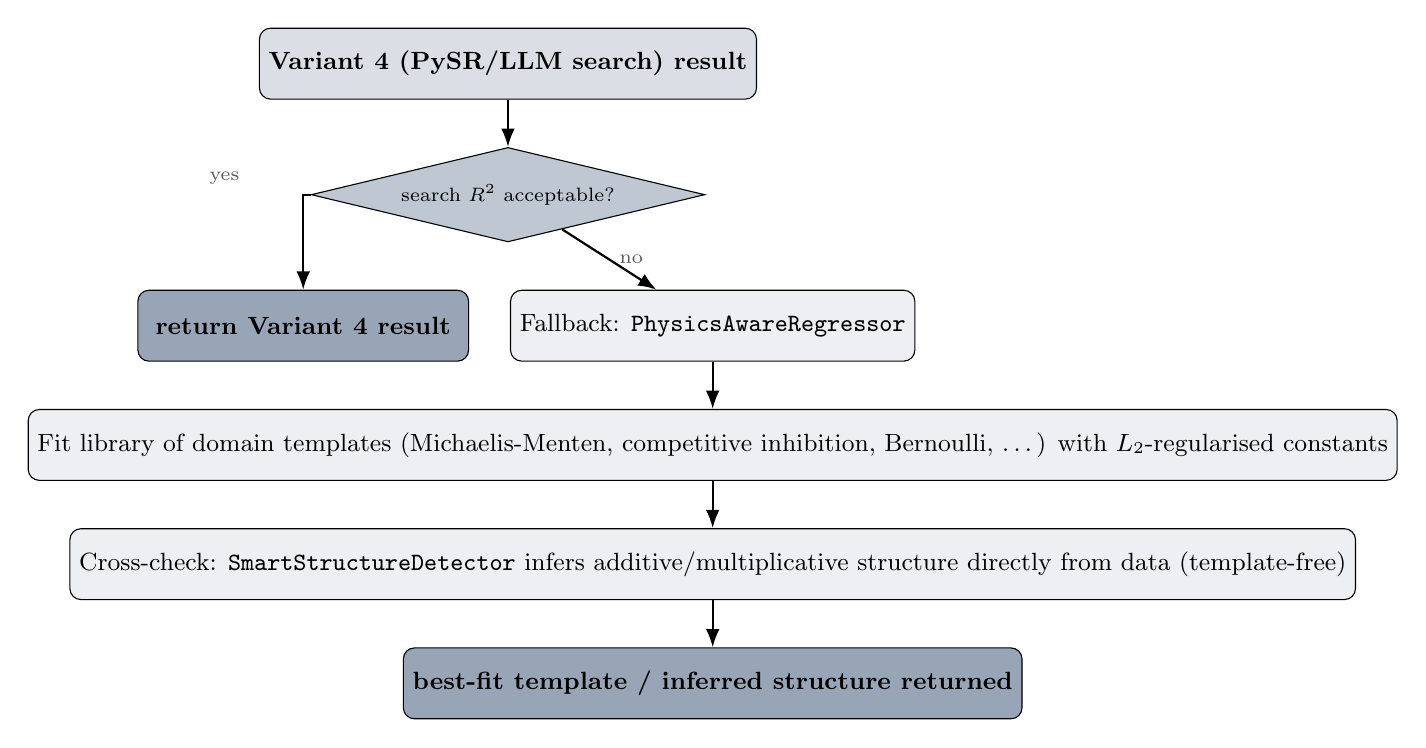
\begin{tikzpicture}[node distance=0.6cm and 1.2cm]
  \node[stage] (s1) {Variant 4 (PySR/LLM search) result};
  \node[dec, below=of s1, minimum width=5.0cm] (d1) {search $R^2$ acceptable?};
  \node[outp, below=of d1, xshift=-2.6cm] (o1) {return Variant 4 result};
  \node[proc, below=of d1, xshift=2.6cm] (s2) {Fallback: \code{PhysicsAwareRegressor}};
  \node[proc, below=of s2] (s3) {Fit library of domain templates (Michaelis-Menten, competitive inhibition, Bernoulli, \ldots) with $L_2$-regularised constants};
  \node[proc, below=of s3] (s4) {Cross-check: \code{SmartStructureDetector} infers additive/multiplicative structure directly from data (template-free)};
  \node[outp, below=of s4] (o2) {best-fit template / inferred structure returned};
  \draw[arr] (s1) -- (d1);
  \draw[arr] (d1) -| node[lbl, above, xshift=-1.0cm]{yes} (o1);
  \draw[arr] (d1) -- node[lbl, right]{no} (s2);
  \draw[arr] (s2) -- (s3);
  \draw[arr] (s3) -- (s4);
  \draw[arr] (s4) -- (o2);
\end{tikzpicture}
\end{center}

\newpage
% ==================================================================
\section{Summary}
% ==================================================================
\begin{center}
\renewcommand{\arraystretch}{1.25}
\begin{tabular}{@{}p{2.9cm}p{4.6cm}p{4.0cm}p{3.1cm}@{}}
\toprule
\textbf{Variant} & \textbf{Combination rule} & \textbf{Domain} & \textbf{Experiments} \\
\midrule
1. Enhanced Hybrid DeFi & threshold gate + scipy refit & DeFi & \code{run\_comparative\_suite\_*}, \code{run\_noise\_sweep\_*}, \code{run\_sample\_complexity\_*}, \code{test\_enhanced\_defi\_*} \\
2. Hybrid All-Domains & tie-favours-symbolic gate + \code{force\_llm} override & Physics/Chem/Bio & \code{run\_comparative\_suite\_*}, \code{run\_sample\_complexity\_*} \\
3. Ensemble Example & inverse-residual-std weighting & DeFi (demo, but used) & \code{hypatiax\_defi\_benchmark\_v3/v4[\_pca]}, \code{test\_enhanced\_defi\_*} \\
4. LLM-Prior / PySR family & 4 modes: none/seed/hybrid/fallback & Nguyen/Feynman & \code{hypatia.py}, \code{exp1\_ablation}, \code{exp1\_five\_system}, \code{exp3\_nguyen12\_*}, \code{run\_comparative\_suite\_*} \\
5. Template physics fallback & template-library or template-free structure fit & Biology/Chem/Eng. & transitively via Variant 4's driver (\code{exp1\_ablation}, \code{run\_comparative\_suite\_*}) \\
\bottomrule
\end{tabular}
\end{center}

\vspace{0.4cm}
\noindent\textit{This report was produced from static reading of the source
files in \repolink\ (fetched from \code{master}); no code in the repository
was executed. Diagrams are faithful redrawings of the control flow as read
from source, not renderings of any runtime trace.}

\end{document}
